\documentclass[journal,12pt,twocolumn]{IEEEtran}
\usepackage{amsmath}
\usepackage{amssymb}
\usepackage{enumerate}
\usepackage[utf8]{inputenc}
\usepackage{multicol}
\usepackage{gensymb}
\usepackage{mathtools}
\usepackage[nice]{nicefrac}
%\usepackage{graphicx}
\usepackage{iithtlc}
%\graphicspath{ {/home/diparna/Documents/optimization} }



\begin{document}

\title{
\logo{
GATE Problems on Optimization
}
}
%\centering \textbf{\Large Optimization}\\
%\bigskip

\maketitle

\begin{enumerate}
\setlength\itemsep{1em}

\item A transportation problem for which the costs, origin and availabilities, destination and requirements are given as follows:\\
\bigskip

\begin{center}
\begin{tabular}{c|c c c|c}
 & $D_1$ & $D_2$ & $D_3$\\ \hline
$Q_1$ & 2 & 1 & 2 & 40\\
$Q_2$ & 9 & 4 & 7 & 60\\
$Q_3$ & 1 & 2 & 9 & 10\\ \hline
 & 40 & 50 & 20\\
\end{tabular}
\end{center}
\bigskip
Check whether the following basic feasible solution
\begin{align*}
x_{11}&=20,x_{13}=20,x_{21}=10,x_{22}=50
\\
x_{33}&=10 \text{ and } x_{12}=x_{23}=x_{32}=x_{33}=0
\end{align*}
is optimal. If not, find an optimal solution.
%
\item The objective function of the dual problem for the following primal linear programming problem: \\ \medskip
Maximize $f=2x_1\!+\!x_2$\\ \medskip
Subject to
\begin{align*}
x_1\!-\!2x_2\! \geqslant\! 2, \\ 
x_1\!+\!2x_2\!=\!8,\\
x_1\!-\!x_2\! \leqslant \! 11,
\end{align*} \\
with $x_1\! \geqslant\!0$ and $x_2$ unrestricted in sign, is given by
%
\begin{enumerate}[(A)]
\begin{multicols}{2}
\setlength\itemsep{1em}
{\small
\item minimize 
$
\!
\begin{aligned}[t]
\text{z}=2y_1 
\\
- \!8y_2\!+\!11y_3
\end{aligned}
$
\item minimize 
$
\!
\begin{aligned}[t]
\text{z} = 2y_1
\\
+ 8y_2\!+\!11y_3
\end{aligned}
$
\item minimize 
$
\begin{aligned}[t]
\text{z}= 2y_1
\\
\!-\! 8y_2\!-\!11y_3
\end{aligned}
$
\item minimize 
$
\begin{aligned}[t]
\text{z} = 2y_1
\\
\!+\!8y_2\!-\!11y_3
\end{aligned}
$
}
\end{multicols}
\end{enumerate}

\item Solve the following linear programming problem using the Simplex method:\\
Minimize $\text{f} = -40x_1\!-\!100x_2$\\
Subject to 
\\
$10x_1 \! + \! 5x_2 \! \leqslant \! 2500$, \\
$4x_1 \! + \! 10x_2 \! \leqslant \! 2000$, \\
$2x_1 \! + \! 3x_2 \! \leqslant \! 900$, \\
$x_1 \! \geqslant \! 0,\! x_2 \! \geqslant \! 0$. 

\item Consider the primal problem (LP) \\
max $4x_1 \! + \! 3x_2$ \\
subject to\\
$x_1 \! + \! x_2 \! \leqslant \! 8$ \\
$2x_1 \! + \! x_2 \! \leqslant \! 10$ \\
$x_1 \! \geqslant \! 0, x_2 \! \geqslant \! 10$ \\
together with its dual (LD).Then 
%
\begin{enumerate}[(A)]
\begin{multicols}{2}
\setlength\itemsep{0.5em}
%{\scriptsize
\item (LP) and (LD) 
\\
both 
are infeasible.
\item (LP) and (LD) 
\\
both are feasible.
\item (LP) is feasible 
but (LD) is infeasible.
\item (LP) is infeasible but (LD) is feasible.
%}
\end{multicols}
\end{enumerate}
%
\item Let \textbf{Z*} denote the optimal value of LPP \\
max $\text{Z} = 4x_1 \! + \! 6x_2 \! + \! 2x_3$\\
such that \\
$3x_1 \! + \! 2x_2 \! + \! x_3 \! = \! 12$ \\
$x_1 \! \geqslant \! 0$, \! $x_2 \! \geqslant \! 0$, \! $x_3 \! \geqslant \! 0$.\\
\medskip
Then 
\begin{enumerate}[(A)]
\begin{multicols}{2}
\setlength\itemsep{1em}
\item $10 \! \leqslant \! \text{Z*} \! \leqslant \! 20$
\item $20 \! < \! \text{Z*} \! \leqslant \! 30$
\item $30 \! < \! \text{Z*} \! \leqslant \! 40$
\item $\text{Z*} \! > \! 40$
\end{multicols}
\end{enumerate}
%
\item Let x be a non-optimal feasible solution of a linear programming maximization problem and y a dual feasible solution. Then
%
\begin{enumerate}[(A)]
\setlength\itemsep{1em}

\item The primal objective value at x is greater than the dual objective value at y.
\item The primal objective value at x could equal the dual objective value at y.
\item The primal objective value at x is less than the dual objective value at y.
\item The dual could be unbounded.

\end{enumerate}

\item Consider the Linear Program \\

\begin{center}
\begin{align*}
\text{Max} \! \sum_{i=1}^{4} c_ix_i ,
\end{align*}
\end{center}
subject to 
%
\begin{align*}
\sum_{i=1}^{4} a_ix_i \; \leqslant \! a_0, \\
0 \! \leqslant \! x_1, \! x_2, \! x_3, \! x_4 \! \leqslant \! 1.
\end{align*}
where $a_i \! > \! 0, \! c_i \! > \! 0$ for $i = 1,2,3,4$ and $a_0 \! > \! 0$ 
%
\begin{enumerate}[(i)]
\setlength\itemsep{1em}

\item Write the dual of this Linear Programming Problem.
\item Assuming 
\begin{align*}
\dfrac{c_1}{a_1} \! \geqslant \! \dfrac{c_2}{a_2} \! \geqslant \! \dfrac{c_3}{a_3} \! \geqslant \! \dfrac{c_4}{a_4}, \\
a_1 \! + \! a_2 \! \leqslant \! a_0, \text{ and } a_1 \! + \! a_2 \! + \! a_3 \! > \! a_0,
\end{align*}
\end{enumerate}
show that the feasible solution 
\begin{align*}
x_1=x_2=1, \! x_3=\frac{a_0-a_1-a_2}{a_3}, \! x_4=0,
\end{align*}
is an optimal solution.

\item Consider the optimal assignment problem, in which n persons $P_1,P_2,.....,P_n$ are to be assigned n jobs $J_1,J_2,.....,J_n$ and where the effectiveness rating of the person $P_i$ for the job $J_j$ is $a_{ij}>0$. The objective is to find an assignment of persons to jobs, that is, a permutation $\sigma : \{1,2,...,n\} \rightarrow \{1,2,...,n\}$ which assigns person $P_i$ to job $J_{\sigma (i)}$, so as to maximize the total effectiveness $\sum_{i=1}^4 \alpha_{i \sigma (i)}$. Show that in any optimal assignment, at least one person is assigned a job at which he is best.

\item Suppose that the linear programming problem $P:\text{Min z} = c^1 \; x \; s.t. \; A_x \! \geqslant \! b,x \! \geqslant \! 0$, where A is an $m \times n$ matrix, c an $n \times 1$ vector and b an $m \times 1$ vector, is being solved by the dual Simplex Algorithm. Then \\

\begin{enumerate}[(A)]
\setlength\itemsep{1em}

\item the value of the primal objective function increases at every iteration
\item the algorithm will always terminate with an optimal solution for the dual
\item the algorithm will always terminate with an optimal solution to the primal
\item it is not always possible to obtain a starting basis for this algorithm
\end{enumerate}

\item Consider the transportation problem given below. The bracketed elements in the table indicate a feasible solution and the elements on the left hand corner are the costs $c_{ij}$ 
\begin{figure}[!h]
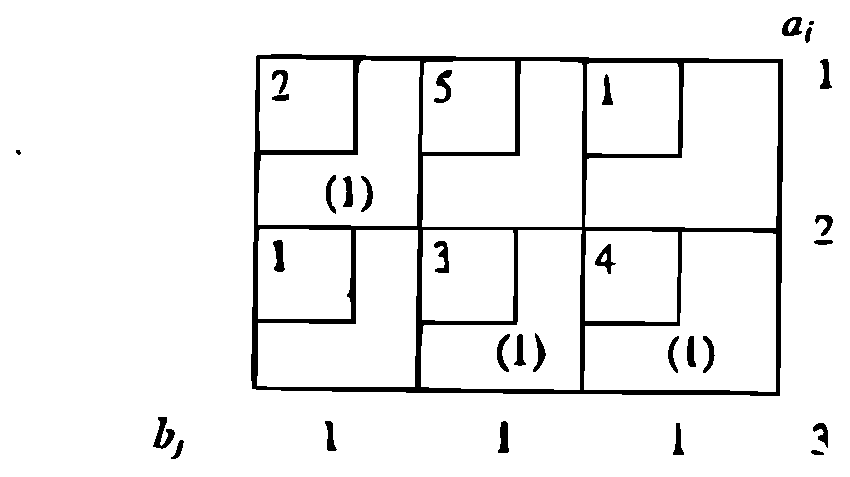
\includegraphics[width=\columnwidth]{figure1.eps}
\label{fig:figure1}
\end{figure}
%
\begin{enumerate}[(A)]
\setlength\itemsep{1em}

\item this solution is a basic feasible solution
\item this solution can be made basic feasible
\item this is an optimal solution
\item the problem does not have an optimal solution

\end{enumerate}

\item Consider the linear programming formulation (P2) of optimally assigning n men to n jobs with respect to some costs $\{c_{ij}\}_{ij=1}^n$. Let A denote the coefficient matrix of the constraint set. Then,

\begin{enumerate}[(A)]
\setlength\itemsep{1em}

\item rank of A is 2n-1 and every basic feasible solution of P2 is integer valued.
\item rank of A is 2n-1 and every basic feasible solution of P2 is not integer valued.
\item rank of A is 2n and every basic feasible solution of P2 is integer valued.
\item rank of A is 2n and every basic feasible solution of P2 is not integer valued.

\end{enumerate}

\item Simplex tableau for phase I of the simplex algorithm for a linear programming problem is given below ($x_3, \! x_4, \! x_5$ are artifical variables): \\
\bigskip

\begin{tabular}{|c|c|c|c|c|c|c|} \hline
Basis & $x_1$ & $x_2$ & $x_3$ & $x_4$ & $x_5$ & RHS \\ \hline
$Z_j-C_J$ & 0 & 0 & -2 & -2 & 0 & 0 \\ 
$x_1$ & 1 & 0 & $\nicefrac{3}{5}$ & $\nicefrac{1}{5}$ & 0 & 2 \\
$x_2$ & 0 & 1 & $\nicefrac{-2}{5}$ & $\nicefrac{1}{5}$ & 0 & 0 \\
$x_3$ & 0 & 0 & -1 & -1 & 1 & 0 \\ \hline
\end{tabular}
\\
\bigskip
Choose the correct statement

\begin{enumerate}[(A)]
\setlength\itemsep{1em}

\item the tableau does not show the end of phase I, since the artifical variable $x_5$ is in the basis
\item the tableau does show the end of phase I, since the value of the phase I objective function is zero
\item the constraints for the original linear programming problem are not redundant
\item the original linear programming problem does not have a feasible solution

\end{enumerate}

\item Given below is the final tableau of a linear programming problem ($x_4$ and $x_5$ are slack variables): \bigskip

\begin{tabular}{|c|c|c|c|c|c|c|} \hline
Basis & $x_1$ & $x_2$ & $x_3$ & $x_4$ & $x_5$ & RHS \\ \hline
$\text{Z}_j- \text{C}_J$ & 0 & 0 & 3 & 5 & 1 & 8 \\
$x_1$ & 1 & 0 & 1 & 4 & -1 & 2 \\
$x_2$ & 0 & 1 & 2 & -1 & 1 & 3 \\ \hline
\end{tabular}
\\
\bigskip
If the right hand side vector $\dfrac{1}{3}$ of the problem gets changed to $\dfrac{1+\theta}{3}$, then the current basic feasible solution is optimal for
\begin{enumerate}[(A)]
\begin{multicols}{2}
\setlength\itemsep{1em}

\item all $\theta \! \leqslant \! 2$
\item all $\theta \! \geqslant \! {-\frac{1}{4}}$
\item all $\theta \in \bigg[{-\dfrac{1}{2}},2 \bigg]$
\item no non-zero value of $\theta$
\end{multicols}
\end{enumerate}

\item Consider the Linear Programming Problem (LPP):\\
Maximize $x_1$,\\
subject to: $3x_1 \! + 4x_2 \! \leqslant \! 10$, $5x_1 \! - \! 2x_2 \! \geqslant \! -2$, $x_1 \! - \! 3x_2 \! \leqslant \! 3$, $x_1, \! x_2 \! \geqslant \! 0$. \\
The value of the LPP is \\
\begin{enumerate}[(A)]
\begin{multicols}{4}
\setlength\itemsep{1em}
\item $\dfrac{9}{5}$
\item 2
\item 3
\item $\dfrac{10}{3}$
\end{multicols}
\end{enumerate}

\item The unit cost $\text{c}_{ij}$ of producing i at plant j is given by the matrix : \\
\medskip
\[\begin{pmatrix}
14&12&16 \\
21&9&17 \\
9&7&5 \\
\end{pmatrix}\]
\medskip
The total cost of optimal assignment is \\

\begin{enumerate}[(A)]
\begin{multicols}{2}
\setlength\itemsep{2em}

\item 20
\item 22
\item 25
\item 28
\end{multicols}
\end{enumerate}

\item Consider the following primal Linear Programming Problem (LPP).\\
Maximize $\text{z} \! = \! 3x_1 \! + \! 2x_2$ \\ \medskip
subject to $x_1 \! - \! x_2 \! \leqslant \! 1$ \\ \medskip
$x_1 \! + \! x_2 \! \geqslant \! 3$ \\ \medskip
$x_1, \! x_2 \! \geqslant \! 0$\\ \medskip
The dual of this problem has 

\begin{enumerate}[(A)]
\begin{multicols}{2}
\setlength\itemsep{1em}
\item infeasible \\ optimal solution
\item unbounded \\ optimal objective value
\item a unique optimal solution
\item infinitely many optimal solutions
\end{multicols}
\end{enumerate}

\item The cost matrix of a Transportation Problem is given by \\ \medskip

\begin{tabular}{|c|c|c|c|} \hline
6 & 4 & 1 & 5 \\ \hline
8 & 9 & 2 & 7 \\ \hline
4 & 3 & 6 & 2 \\ \hline
\end{tabular}
\medskip
The following values of the basic variables were obtained at the first iteration: \\ \smallskip
$x_{11} \! = \! 6$, $x_{12} \! = \! 8$, $x_{22} \! = \! 2$, $x_{23} \! = \! 14$, $x_{33} \! = \! 1$, $x_{34} \! = \! 4$. \\
\smallskip
Then \\
\begin{enumerate}[(A)]
\setlength\itemsep{1em}
\item the current solution is optimal
\item the current solution is nonoptimal and the entering and leaving variables are $x_{31}$ and $x_{33}$ respectively
\item the current solution is nonoptimal and the entering and leaving variables are $x_{21}$ and $x_{12}$ respectively
\item the current solution is nonoptimal and the entering and leaving variables are $x_{14}$ and $x_{12}$ respectively.
\end{enumerate}

\item In a balanced transportation problem, if all the unit transportation costs $c_{ij}$, are decreased by a nonzero constant $a$, then in the optimal solution of the revised problem \\
\begin{enumerate}[(A)]
\setlength\itemsep{1em}
\item the values of the decision variables and the objective value remain unchanged
\item the values of the decision variables change but the objective value remains unchanged
\item the values of the decision variables remain unchanged but the objective value changes
\item the value of the decision variables and the objective value change.
\end{enumerate}

\item Consider the following Linear Programming Problem (LPP).\\
Maximize $\text{z} \! = \! 3x_1 \! + \! x_2$ \\
subject to $x_1 \! + \! 2x_2 \! \leqslant \! 5$\\
$x_1 \! + \! x_2 \! - \! x_3 \! \leqslant \! 2$\\
$7x_1 \! + \! 3x_2 \! - \! 5x_3 \! \leqslant \! 20$\\
$x_1, \! x_2, \! x_3 \! \geqslant \! 0$. \\
\smallskip
The nature of the optimal solution to the problem is
\begin{enumerate}[(A)]
\begin{multicols}{2}
\setlength\itemsep{1em}

\item nondegenerate \\ alternative optima
\item degenerate \\ alternative optima
\item degenerate unique optimal
\item nondegenerate unique optimal
\end{multicols}
\end{enumerate}

\item For a linear programming primal maximization problem P with dual Q, which of the following statements is correct?
\begin{enumerate}[(A)]
\setlength\itemsep{1em}
\item The optimal values of P and Q exist and are the same
\item Both optimal values exist and the optimal value of P is less than the optimal value of Q
\item P will have an optimal solution, if and only if Q also has an optimal solution
\item Both P and Q cannot be feasible
\end{enumerate}

\item Let a convex set in 9-dimensional space be given by the solution set of the following system of linear inequalities
\begin{center}
\begin{align*}
\sum_{i=1}^{3} \text{x}_{ij} = 1,  \quad  i = 1,2,3 \\
\sum_{j=1}^{3} \text{x}_{ij} = 1,  \quad  j = 1,2,3 \\
x_{ij} \geqslant 0, \quad i,j = 1,2,3    
\end{align*}
\end{center}
\smallskip
Then, the number of extreme points of this set is
\begin{enumerate}[(A)]
\begin{multicols}{2}
\setlength\itemsep{1em}
\item 3
\item 4
\item 9
\item 6
\end{multicols}
\end{enumerate}

\item Consider the linear programming problem 
\begin{center}
\begin{align*}
\text{Max} \; c_1x_1 \! + \! c_2x_2 \! + \! c_3x_3 \\
\text{s.t} \; x_1 \! + \! x_2 \! + \! x_3 \! \leqslant \! 4 \\
x_1 \! \leqslant \! 2 \\
x_3 \! \leqslant \! 3 \\
3x_1 \! + \! x_3 \! \leqslant \! 7 \\
x_1, \! x_2, \! x_3 \! \geqslant \! 0.
\end{align*}
\end{center}
\smallskip
If (1,0,3) is an optimal solution, then
\begin{enumerate}[(A)]
\begin{multicols}{2}
\setlength\itemsep{1em}
\item $c_1 \! \leqslant \! c_2 \! \leqslant c_3$
\item $c_3 \! \leqslant \! c_1 \! \leqslant \! c_2$
\item $c_2 \! \leqslant \! c_3 \! \leqslant \! c_1$
\item $c_2 \! \leqslant \! c_1 \! \leqslant \! c_3$

\end{multicols}
\end{enumerate}

\item Let the convex set S be given by the solution set of the following system of linear inequalities in the sixteen variables $\{ x_{ij} \! : \! i,j \! = \! 1,......,4\}:$\\
\begin{center}
\begin{align*}
\sum_{i=1}^{4} x_{ij} \! = \! 3, \quad i = 1,....,4 \\
\sum_{j=1}^{4} x_{ij} \! = \! 3, \quad j=1,....,4. \\
x_{ij} \! \geqslant \! 0, \quad i,j=1,...,4.
\end{align*}
\end{center}
Then, the dimension of S is equal to
\begin{enumerate}[(A)]
\begin{multicols}{2}
\setlength\itemsep{1em}
\item 4
\item 9
\item 8
\item 12 \\
\end{multicols}
\end{enumerate}

\textbf{\underline{Data for the following two questions:}} \\
\medskip
Consider the Linear Programming Problem P: 
\begin{align*}
\text{Max} \; c_1x_1 \! + \! c_2x_2 \! + \! ......+ \! c_nx_n \\
\text{s.t.} \sum_{i=1}^{n} a_{ij}x_j \! \leqslant \! b_i, \quad i=1,...,m, \\
x_j \! \geqslant \! 0, \quad j=1,...,n, 
\end{align*}
with m constraints in n non-negative variables.\\

\item Let $x^* \! = \! (x_1^*, \! x_2^*, \! .....,x_n^*)$ be an optimal extreme point solution to P with $x_1^*, \! x_2^*, \! x_3^*,.....,x_n^* \! > \! 0$. Then, out of the m constraints $\sum_{j=1}^{n} a_{ij}x_j \! \leqslant \! b_i, \quad i=1,...,m$, the number of constraints not satisfied with equality at $x^*$ is 

\begin{enumerate}[(A)]
\begin{multicols}{2}
\setlength\itemsep{1em}
\item at most $m \! - \! 4$
\item at most $n \! - \! 4$
\item equal to $m \! - \! 3$
\item equal to $m \! - \! 2$
\end{multicols}
\end{enumerate}

\item Treat $c_i$'s, $a_{ij}$'s as fixed and consider the problem P for different values of $b_i$'s. Let P be unbounded for some set of parameters $b_1, \! b_2,...., \! b_m$. Then 
\begin{enumerate}[(A)]
\setlength\itemsep{1em} 

\item $n \! > \! m$
\item P is either unbounded or infeasible for every choice of $b_i$'s
\item $m \! > \! n$
\item P has an optimal solution for some choice of $b_i$'s.
\end{enumerate} 

\item Consider the linear programming problem, \\
max $\text{z} \! = \! c_1x_1 \! + \! c_2x_2, \! c_1, \! c_2 \! > 0$ \\
Subject to $x_1 \! + \! x_2 \! \leqslant \! 3$ \\ \medskip
$2x_1 \! + \! 3x_2 \! \leqslant \! 4$ \\
$x_1, \! x_2 \! \geqslant \! 0$. \\
Then,

\begin{enumerate}[(A)]
\setlength\itemsep{1em}
\item The primal has an optimal solution but the dual does not have an optimal solution.
\item Both the primal and the dual have optimal solutions
\item The dual has an optimal solution but the primal does not have an optimal solution
\item Neither the primal nor the dual have optimal solutions.
\end{enumerate}

\item For each $a \! \in \! \mathbb{R}$, consider the linear programming problem \\
Max $\text{z} \! = \! x_1 + \! 2x_2 \! + \! 3x_3 \! + \! 4x_4$\\
subject to 
\begin{align*}
ax_1 \! + \! 2x_2 \! \leqslant \! 1 \\
x_1 \! + \! ax_2 \! + \! 3x_4 \! \leqslant \! 2 \\
x_1, \! x_2, \! x_3, \! x_4 \! \geqslant \! 0 
\end{align*}
Let S \{ $a \! \in \! \mathbb{R}$: the given LP problem has a basic feasible solution\}. Then 
\begin{enumerate}[(A)]
\begin{multicols}{2}
\setlength\itemsep{1em}
\item $\text{S} \! = \! \phi$
\item S = R
\item $\text{S} = (0, \infty)$
\item $\text{S} = (-\infty, 0)$
\end{multicols}
\end{enumerate}

\item Consider the linear programming problem \\
Max $\text{z} \! = \! x_1 \! + \! 5x_2 \! + \! 3x_3$ \\
subject to \\
\begin{center}
\begin{align*}
2x_1 \! - \! 3x_2 \! + \! 5x_3 \! \leqslant \! 3 \\
3x_1 \! + \! 2x_3 \! \leqslant \! 5 \\
x_1, \! x_2, \! x_3 \! \geqslant \! 0.
\end{align*}
\end{center}
Then the dual of this LP problem 
\begin{enumerate}[(A)]
\setlength\itemsep{1em}
\item has a feasible solution but does not have a basic feasible soliution
\item has a basic feasible solution
\item has infinite number of feasible solutions
\item has no feasible solution
\end{enumerate}

\item Let $c_{ij} \! \geqslant \! 2$ be the cost of the $(i,j)^{th}$ cell of an assignment problem. If a new cost matrix is generated by the elements $c_{ij}^{.} \! = \! \frac{1}{2}c_{ij} \! + \! 1$, then
\begin{enumerate}[(A)]
\setlength\itemsep{1em}
\item optimal assignment plan remains unchanged and cost of assignment decreases
\item optimal assignment plan changes and cost of assignment decreases
\item optimal assignment plan remains unchanged and cost of assignment increases
\item optimal assignment plan changes and cost of assignment increases
\end{enumerate}

\item Let a primal linear programming admit an optimal solution. Then the corresponding dual problem
\begin{enumerate}[(A)]
\setlength\itemsep{1em}
\item does not have a feasible solution
\item has a feasible solution but does not have any optimal solution
\item does not have a convex feasible region
\item has an optimal solution
\end{enumerate}

\item The cost matrix of a transportation problem is given by \\
\medskip
\begin{tabular}{|c|c|c|c|} \hline
1 & 2 & 3 & 4 \\ \hline
4 & 3 & 2 & 0 \\ \hline
0 & 2 & 2 & 1 \\ \hline
\end{tabular}
\\
\medskip
The following are the values of variables in a feasible solution \\
$x_{12} \! = \! 6$, $x_{23} \! = \! 2$, $x_{24} \! = \! 6$, $x_{31} \! = \! 4$, $x_{33} \! = \! 6$ \\
\medskip
Then which of the following is correct??
\begin{enumerate}[(A)]
\setlength\itemsep{1em}
\item The solution is degenerate and basic
\item The solution is non-degenerate and basic
\item The solution is degenerate and non-basic
\item The solution is non-degenerate and non-basic
\end{enumerate}

\item The maximum value of $\text{z} \! = \! 3x_1 \! - \! x_2$ subject to $2x_1 \! - \! x_2 \! \leqslant \! 1$, $x_1 \! \leqslant \! 3$ and $x_1, \! x_2 \! \geqslant \! 0$ is
\begin{enumerate}[(A)]
\begin{multicols}{4}
\setlength\itemsep{1em}
\item 0
\item 4
\item 6
\item 9
\end{multicols}
\end{enumerate}

\item Consider the problem of maximizing $\text{z} \! = \!2x_1 \! + \! 3x_2 \! - \! 4x_3 \! + \! x_4$ subject to 
\begin{align*}
x_1 \! + \! x_2 \! + \! x_3 \! = \! 2, \\
x_1 \! - \! x_2 \! + \! x_3 \! = \! 2, \\
2x_1 \! + \! 3x_2 \! + 2x_3 \! - \! x_4 \! = \! 0, \\
x_1, \! x_2, \! x_3, \! x_4 \! \geqslant \! 0. 
\end{align*}
\medskip
Then 
\begin{enumerate}[(A)]
\setlength\itemsep{1em}
\item (1,0,1,4) is a basic feasible solution but (2,0,0,4) is not
\item (1,0,1,4) is not a basic feasible solution but (2,0,0,4) is
\item neither (1,0,1,4) nor (2,0,0,4) is a basic feasible solution
\item both of (1,0,1,4) and (2,0,0,4) are basic feasible solutions
\end{enumerate}

\item Which one of the following is TRUE??
\begin{enumerate}[(A)]
\setlength\itemsep{1em} 
\item Every linear programming problem has a feasible solution.
\item If a linear programming problem has an optimal solution then it is unique.
\item The union of two convex sets is necessarily convex.
\item Extreme points of the $x^2 \! + \! y^2 \! \leqslant \! 1$ are the point on the circle $x^2 \! + \! y^2 \! = \! 1$.
\end{enumerate}

\item The dual of the linear programming problem \\
Minimize $c^{\tau}x$ subject to $Ax \! \geqslant \! b$ and $x \! \geqslant \! 0$ is 
\begin{enumerate}[(A)]
\setlength\itemsep{1em}
\item Maximize $b^{\tau}w$ subject to $A^{\tau}w \! \geqslant \! c$ and $w \! \geqslant \! 0$
\item Maximize $b^{\tau}w$ subject to $A^{\tau}w \! \leqslant \! c$ and $w \! \geqslant \! 0$
\item Maximize $b^{\tau}w$ subject to $A^{\tau}w \! \leqslant \! c$ and w is unrestricted
\item Maximize $b^{\tau}w$ subject to $A^{\tau}w \! \geqslant \! c$ and w is unrestricted
\end{enumerate}

\item The minimum value of \\
$\text{z} \! = \! 2x_1 \! - \! x_2 \! + \! x_3 \! - \! 5x_4 \! + \! 22x_5$ subject to 
\begin{align*}
x_1 \! - \! 2x_4 \! + \! x_5 \! = \! 6 \\
x_2 \! + \! x_4 \! - \! 4x_5 \! = \! 3 \\
x_3 \! + \! 3x_4 \! + \! 2x_5 \! = \! 10 \\
x_j \! \geqslant \! 0, \quad j=1,2,....,5 
\end{align*} 
is 
\begin{enumerate}[(A)]
\begin{multicols}{4}
\setlength\itemsep{1em}
\item 28
\item 19
\item 10
\item 9
\end{multicols}
\end{enumerate}

\item Using the Hungarian method, the optimal value of the assignment problem whose cost matrix is given by \\
\medskip
\begin{tabular}{|c|c|c|c|} \hline
5 & 23 & 14 & 8 \\ \hline
10 & 25 & 1 & 23 \\ \hline
35 & 16 & 15 & 12 \\ \hline
16 & 23 & 11 & 7 \\ \hline
\end{tabular}
\\
\medskip
is
\begin{enumerate}[(A)]
\begin{multicols}{4}
\setlength\itemsep{1em}
\item 29
\item 52
\item 26
\item 44
\end{multicols}
\end{enumerate}

\item The following table gives the cost matrix of a transportation problem \\
\medskip
\begin{tabular}{|c c c|} \hline
4 & 5 & 6 \\
3 & 2 & 2 \\
1 & 1 & 2 \\ \hline
\end{tabular}
\\
\medskip
The basic feasible solution given by $x_{11} \! = \! 3$, $x_{13} \! = \! 1$, $x_{23} \! = \! 6$, $x_{31} \! = \! 2$, $x_{32} \! = \! 5$ is
\begin{enumerate}[(A)]
\setlength\itemsep{1em}
\item degenerate and optimal
\item optimal but not degenerate
\item degenerate but not optimal
\item neither degenerate nor optimal
\end{enumerate}

\item If $\text{z}^{*}$ is the optimal value of the linear programming problem \\
Maximize $\text{z} \! = \! 5x_1 \! + \! 9x_2 \! + \! 4x_3$ \\
subject to $x_1 \! + \! x_2 \! + \! x_3 \! = \! 5$ \\
$4x_1 \! + \! 3x_2 \! + \! 2x_3 \! = \! 12$ \\
$x_1, \! x_2, \! x_3 \! \geqslant \! 0$ \\
then
\begin{enumerate}[(A)]
\begin{multicols}{2}
\setlength\itemsep{1em}
\item $0 \! \leqslant \! \text{z}^{*} \! < \! 10$
\item $10 \! \leqslant \! \text{z}^{*} \! < \! 20$
\item $20 \! \leqslant \! \text{z}^{*} \! < \! 30$
\item $30 \! \leqslant \! \text{z}^{*} \! < \! 40$
\end{multicols}
\end{enumerate}

\item The Linear Programming Problem: \\
Maximize $\text{z} \! = \! x_1 + \! x_2$ \\
subject to 
\begin{align*}
x_1 \! + \! 2x_2 \! \leqslant \! 20 \\
x_1 \! + \! x_2 \! \leqslant \! 15 \\
x_2 \! \leqslant \! 6 \\
x_1, \! x_2 \! \geqslant \! 0 
\end{align*}
\begin{enumerate}[(A)]
\begin{multicols}{2}
\setlength\itemsep{1em}
{\small
\item has exactly one \\ optimum solution
\item has more than \\ one optimum solution
\item has unbounded solution
\item has no solution
}
\end{multicols}
\end{enumerate}

\item Consider the Primal Linear Programming Problem: \\
\smallskip
\textbf{P}:
$
\begin{cases}
\text{Maximize} \; \text{z} \! = \! c_1x_1 \! + \! c_2x_2 \! +.....+ \! c_nx_n \\
\text{subject to} \\

a_{11}x_1 \! + \! a_{12}x_2 \! +.....+ \! a_{1n}x_n \! \leqslant \! b_1 \\
a_{21}x_1 \! + \! a_{22}x_2 \! +......+ \! a_{2n}x_n \! \leqslant \! b_2 \\
. \\
. \\
. \\
. \\
. \\
a_{m1}x_1 \! + \! a_{m2}x_2 \! +.....+ \! a_{mn}x_n \! \leqslant \! b_m \\
x_j \! \geqslant \! 0, \quad j=1,....,n. 

\end{cases}
$
\\
\smallskip
The Dual of P is \\
\textbf{D}:
$
\begin{cases}
\text{Minimize} \; \text{z'} \! = \! b_1w_1 \! + \! b_2w_2 \! +.....+ \! b_mw_m \\
\text{subject to} \\

a_{11}w_1 \! + \! a_{12}w_2 \! +.....+ \! a_{m1}w_m \! \leqslant \! c_1 \\
a_{12}w_1 \! + \! a_{22}w_2 \! +......+ \! a_{m2}w_m \! \leqslant \! c_2 \\
. \\
. \\
. \\
. \\
. \\
a_{1n}w_1 \! + \! a_{2n}w_2 \! +.....+ \! a_{mn}w_m \! \leqslant \! c_n \\
w_i \! \geqslant \! 0, \quad i=1,....,m. 

\end{cases}
$
\\
\medskip
Which of the following statements is FALSE?
\begin{enumerate}[(A)]
\setlength\itemsep{1em}
\item IF P has an optimal solution, then D also has an optimal solution
\item The dual of the dual problem is a primal problem
\item If P has an unbounded solution, then D has no feasible solution
\item If P has no feasible solution, then D has a feasible solution
\end{enumerate}

\item We have to assign four jobs I,II,III,IV to four workers A,B,C and D. The time taken by different workers (in hours) in completing different jobs is given below: \\
\begin{table}[!h]
\begin{center}
\begin{tabular}{c c c c c c}
& & I & II & III & IV \\
& A & 5 & 3 & 2 & 8 \\
Workers & B & 7 & 9 & 2 & 6 \\
& C & 6 & 4 & 5 & 7 \\
& D & 5 & 7 & 7 & 8   
\end{tabular}
\end{center}
\end{table}
The optimal assignment is as follows: \\
Job III to worker A; Job IV to worker B; Job II to worker C and Job I to worker D and hence the time taken by different workers in completing different jobs is now changed as: 
\begin{table}[!h]
\begin{center}
\begin{tabular}{c c c c c c}
& & I & II & III & IV \\
& A & 5 & 3 & 2 & 5 \\
Workers & B & 7 & 9 & 2 & 3 \\
& C & 4 & 2 & 3 & 2 \\
& D & 5 & 7 & 7 & 5  
\end{tabular}
\end{center}
\end{table}
Then the minimum time (in hours) taken by the workers to complete all the jobs is 
\begin{enumerate}[(A)]
\begin{multicols}{4}
\setlength\itemsep{1em}
\item 10
\item 12
\item 15
\item 17
\end{multicols}
\end{enumerate}

\item The following table shows the information on the availability of supply to each warehouse, the requirement of each market and unit of transportation cost (in rupees) from each warehouse to each market.
%\medskip
\begin{table}[!h]
\centering
\begin{tabular}{c c c c c c c}
& & Market & & & & \\
& & $M_1$ & $M_2$ & $M_3$ & $M_4$ & Supply \\
& $W_1$ & 6 & 3 & 5 & 4 & 22 \\
Warehouse & $W_2$ & 5 & 9 & 2 & 7 & 15 \\
& $W_3$ & 5 & 7 & 8 & 6 & 8 \\
Requirement & & 7 & 12 & 17 & 9 & 
\end{tabular}
\end{table}
\medskip
The present transportation schedule is as follows: \\
$W_1$ to $M_2$: 12 units; $W_1$ to $M_3$: 1 unit; $W_1$ to $M_4$: 9 units; $W_2$ to $M_3$: 15 units; $W_3$ to $M_1$: 7 units and $W_3$ to $M_3$: 1 unit. Then the minimum total transportation cost (in rupees) is
\begin{enumerate}[(A)]
\begin{multicols}{4}
\setlength\itemsep{1em}
\item 150
\item 149
\item 148
\item 147
\end{multicols}
\end{enumerate}

\item Consider the linear programming problem: \\

Maximize \quad $x \! + \! \frac{3}{2}y$ 
subject to
\begin{align*}
2x \! + \! 3y \! \leqslant \! 16, \\
x \! + \! 4y \! \leqslant \! 18, \\
x \! \geqslant \! 0, \! y \! \geqslant \! 0. 
\end{align*}
%
If S denotes the set of all solutions of the above problem, then 

\begin{enumerate}[(A)]
\begin{multicols}{2}
\setlength\itemsep{1em}
\item S is empty
\item S is a singleton
\item S is a line segement
\item S has positive area
\end{multicols}
\end{enumerate}

\item Consider the following linear programming problem: \\
Maximize $x \! + \! 3y \! + \! 6z \! - \! w$ \\
subject to $5x \! + \! y \! + \! 6z + \! 7w \! \leqslant \! 20$, \\
$6x \! + \! 2y \! + 2z \! + \! 9w \! \leqslant \! 40$, \\
$x \! \geqslant \! 0$, $y \! \geqslant \! 0$, $z \! \geqslant \! 0$, $w \! \geqslant \! 0$. \\
Then the optimal value is .....

\item LEt X be a convex region in the plane bounded by straight lines. Let X have 7 vertices. Suppose $\text{f}(x,y) \! = \! ax \! + \! by \! + \! c$ has maximum value M and minimum value N on X and $\text{N} \! < \! M$. Let S= \{P: P is a vertex of X and N $<$ f(P) $<$ M\}. If S has n elements, then which of the following statements is TRUE?
\begin{enumerate}[(A)]
\begin{multicols}{2}
\setlength\itemsep{1em}
\item n cannot be 5
\item n can be 2
\item n cannot be 3
\item n can be 4
\end{multicols}
\end{enumerate}

\item Consider the following linear programming problem: \\
Minimize $x_1 \! + \! x_2$ \\
Subject to: \\
\begin{center}
\begin{align*}
2x_1 \! + \! x_2 \! \geqslant \! 8 \\
2x_1 \! + \! 5x_2 \! \geqslant \! 10 \\
x_1, \! x_2 \! \geqslant \! 0 
\end{align*}
\end{center}
\medskip
The optimal value to this problem is ........

\item Consider the following linear programming problem: \\
Minimize: $x_1 \! + \! x_2 \! + \! 2x_3$ \\
Subject to
\begin{center}
\begin{align*}
x_1 \! + \! 2x_2 \! \geqslant \!  4 \\
x_2 \! + \! 7x_3 \! \leqslant \! 5 \\
x_1 \! - \! 3x_2 \! + \! 5x_3 \! = \! 6 \\
x_1, \! x_2 \! \geqslant \! 0, \; x_3 \;  \text{is unrestricted} 
\end{align*}
\end{center}
\medskip
The dual to this problem is: \\
Maximize: $4y_1 \! + \! 5y_2 \! + \! 6y_3$ \\
Subject to \\
\begin{center}
\begin{align*}
y_1 \! + y_3 \! \leqslant \! 1 \\
2y_1 \! + y_2 \! - \! 3y_3 \! \leqslant \! 1 \\
7y_2 \! + \! 5y_3 \! = \! 2 
\end{align*}
\end{center}
\smallskip
and further subject to:\\
\begin{enumerate}[(A)]
\setlength\itemsep{1em}
\item $y_1 \! \geqslant \! 0$, $y_2 \! \leqslant \! 0$ and $y_3$ is unrestricted
\item $y_1 \! \geqslant \! 0$, $y_2 \! \geqslant \! 0$ and $y_3$ is unrestricted
\item $y_1 \! \geqslant \! 0$, $y_3 \! \leqslant \! 0$ and $y_2$ is unrestricted
\item $y_3 \! \geqslant \! 0$, $y_2 \! \leqslant \! 0$ and $y_1$ is unrestricted
\end{enumerate}

\item Consider the linear programming problem \\
Maximize $3x \! + \! 9y$, \\
Subject to \\
\begin{center}
\begin{align*}
2y \! - \! x \! \leqslant \! 2 \\
3y \! - \! x \! \geqslant \! 0 \\
2x \! + \! 3y \! \leqslant \! 10 \\
x, \! y \! \geqslant \! 0. 
\end{align*}
\end{center}
\medskip
Then the maximum value of the objective function is equal to ........

\item Minimize $w \! = \! x \! + \! 2y$ subject to \\
\begin{center}
\begin{align*}
2x \! + \! y \! \geqslant \! 3 \\
x \! + \! y \! \geqslant \! 2 \\
x \! \geqslant \! 0, \! y \! \geqslant \! 0 \\
\end{align*}
\end{center}
\smallskip
Then, the minimum value of w is equal to .......

\item Maximize $w \! = \! 11x \! - \! z$ subject to \\
\begin{center}
\begin{align*}
10x \! + \! y \! - \! z \! \leqslant \! 1 \\
2x \! - \! 2y \! + \! z \! \leqslant \! 2 \\
x, \! y, \! z \! \geqslant \! 0. 
\end{align*}
\end{center}
\smallskip
Then, the maximum value of w is equal to ......

\item Consider the linear programming problem (LPP): \\
Maximize $4x_1 \! + \! 6x_2$ \\
Subject to $x_1 \! + \! x_2 \! \leqslant \! 8$, \\
$2x_1 \! + \! 3x_2 \! \geqslant \! 18$, \\
$x_1 \! \geqslant \! 6$, $x_2$ is unrestricted in sign.\\
\smallskip
Then the LPP has \\
\begin{enumerate}[(A)]
\setlength\itemsep{1em}
\item no optimal solution
\item only one basic feasible solution and that is optimal
\item more than one basic feasible solution and a unique optimal solution
\item infinitely many optimal solutions
\end{enumerate}

\item For a linear programming problem (LPP) and its dual, which one of the following is NOT TRUE?
\begin{enumerate}[(A)]
\setlength\itemsep{1em}
\item The dual of the dual is primal
\item If the primal LPP has an unbounded objective function, then the dual LPP is feasible
\item If the primal LPP is infeasible, then the dual LPP must have unbounded objective function
\item If the primal LPP has afinite optimal solution, then the dual LPP also has a finite optimal solution
\end{enumerate}

\item Consider the following transportation problem. The entries inside the cells denote per unit cost of transportation from the origins to the destinations.
\begin{table}[!h]
\begin{center}
\begin{tabular}{c c c c c c}
& & & Destination & & \\
& & 1 & 2 & 3 & Supply \\
& 1 & 4 & 3 & 6 & 20 \\
Origin & 2 & 7 & 10 & 5 & 30 \\
& 3 & 8 & 9 & 7 & 50 \\
& Demand & 10 & 30 & 60 & 
\end{tabular}
\end{center}
\end{table}
The optimal cost of transportation equals .........

\item Consider the linear programming problem (LPP): \\
Maximize $kx_1 \! + \! 5x_2$\\
Subject to $x_1 \! + \! x_2 \! \leqslant \! 1$, \\
$2x_1 \! + \! 3x_2 \! \leqslant \! 1$, \\
$x_1, \! x_2 \! \geqslant \! 0$.\\
\smallskip
If $x^* \! = \! (x_1^*, \! x_2^*)$ is an optimal solution of the above LPP with k=2, then the largest value of k (rounded to 2 decimal places) for which $x^*$ remains optimal equals .........

\end{enumerate}
\end{document}

